\subsection{Assessment of SQL and NoSQL Systems to Store and
Mine COVID-19 Data}

\begin{frame}
    \frametitle{Assessment of SQL and NoSQL Systems to Store and Mine COVID-19 Data}

    Este estudio fue llevado a cabo en el año 2022 por tres investigadores pertenecientes a los siguientes institutos

    \vspace{-0.3cm}
    
    \begin{center}
        \textit{Instituto de Ingeniería de Coimbra}$^1$, \textit{Centro de Informática y Sistemas de la Universidad de Coimbra}$^2$ e \textit{Instituto Tecnológico de São Paulo}$^3$
    \end{center}

    \vspace{-0.4cm}
    
    \begin{center}
        João Antas$^1$, Rodrigo Rocha Silva$^{2,3}$ y Jorge Bernardino$^{1,2}$
    \end{center}

    \vspace{-0.1cm}
    
    y tuvo como objetivo:

     

    \begin{itemize}
        \item Estudiar diferentes sistemas de bases de datos, con el fin de ayudar a seleccionar el más adecuado para almacenar, gestionar y minar datos relacionados con el COVID-19.

         
        
        \item Llevar a cabo un proceso de Minería de Datos, empleando pruebas de clasificación de datos del software Orange Data Mining.
    \end{itemize}

     

    Nos vamos a centrar en mostrar como se logró el primer objetivo.
\end{frame}

\begin{frame}
    \frametitle{Assessment of SQL and NoSQL Systems to Store and Mine COVID-19 Data}

    Para ambos experimentos, utilizaron una computadora con las siguiente características:

     
    
    \begin{itemize}
        \item Windows 10
        \item Procesador Intel Core i7-8750H 2.20GHz
        \item 16 GB de RAM
        \item 256 GB SSD de Almacenamiento
    \end{itemize}

     
    
    Además las versiones de las tecnologías utilizadas fueron las siguientes:

     
    
    \begin{itemize}
        \item SQL Server versión 2017
        \item MongoDB versión 4.4
        \item Cassandra versión 3.11.10
    \end{itemize}
\end{frame}

\begin{frame}
    \frametitle{Assessment of SQL and NoSQL Systems to Store and Mine COVID-19 Data}

    Los datos fueron obtenidos de distintas fuentes, como hospitales, datos públicos, etc., y fueron almacenados en formatos CSV o XML antes de ser incorporados a las bases de datos.   Y para evaluar la escalabilidad de las bases de datos, crearon dos datasets de distintos tamaños. 

     
    
    Para el primer experimento, utilizaron seis queries diferentes, con el objetivo de evaluar el tiempo de ejecución, la RAM utilizada y el porcentaje de CPU de cada consulta. 
    
     
    
    Vamos a mostrar los resultados obtenidos sobre las consultas 1, 2 y 3, que se presentan a continuación.

\end{frame}

\begin{frame}
    \frametitle{Assessment of SQL and NoSQL Systems to Store and Mine COVID-19 Data}

    \begin{figure}[H]
        \begin{center}
            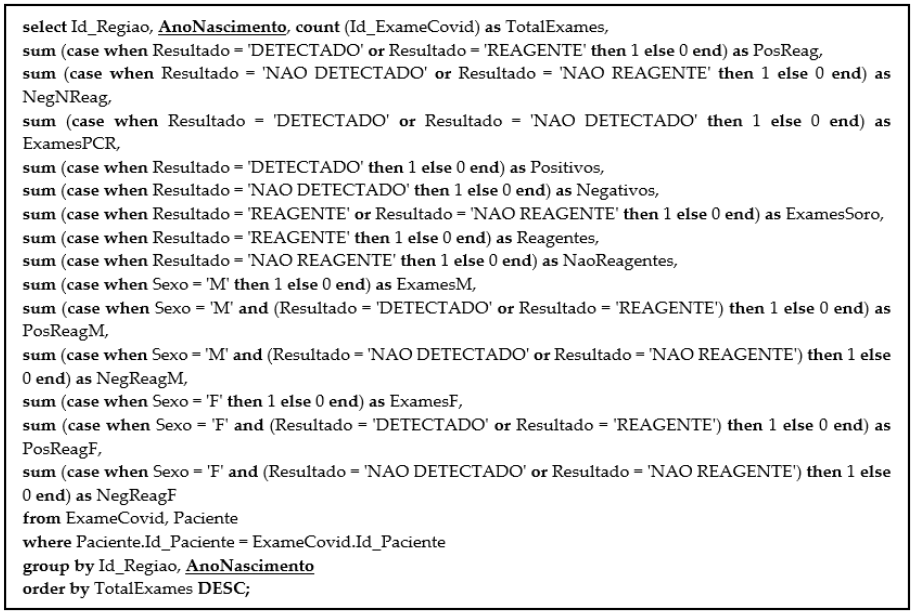
\includegraphics[width=0.7\textwidth]{images/cov19-query12.png}
            \caption{Query Region (Query 1 - sin subrayado) y Query RegionYear (Query 2)}
            \label{cov19-q12}
        \end{center}
    \end{figure}
\end{frame}

\begin{frame}
    \frametitle{Assessment of SQL and NoSQL Systems to Store and Mine COVID-19 Data}

    Esta query fue seleccionada utilizando un registro de auditoría que controlaba todas las consultas realizadas en la base de datos de SQL Server.
    
    \begin{figure}[H]
        \begin{center}
            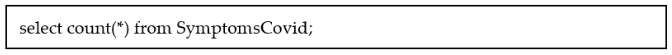
\includegraphics[width=0.82\textwidth]{images/cov19-query3.png}
            \caption{Query de Orange Data Mining (Query 3)}
            \label{cov19-q3}
        \end{center}
    \end{figure}
\end{frame}

\begin{frame}
    \frametitle{Assessment of SQL and NoSQL Systems to Store and Mine COVID-19 Data}

    \begin{figure}[H]
        \centering
        \begin{minipage}[b]{0.48\textwidth}
            \centering
            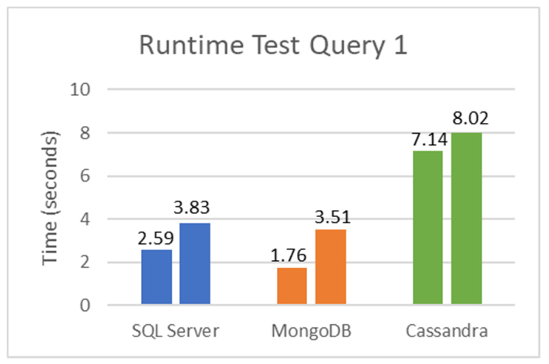
\includegraphics[width=\textwidth]{images/cov19-runt-test-q1.png}
            \caption{Prueba de tiempo de ejecución para la Query 1.}
        \end{minipage}
        \hfill
        \begin{minipage}[b]{0.48\textwidth}
            \centering
            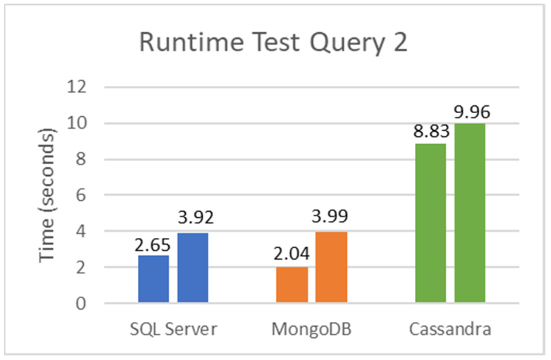
\includegraphics[width=\textwidth]{images/cov19-runt-test-q2.png}
            \caption{Prueba de tiempo de ejecución para la Query 2.}
        \end{minipage}
    \end{figure}
\end{frame}

\begin{frame}
    \frametitle{Assessment of SQL and NoSQL Systems to Store and Mine COVID-19 Data}

    \begin{figure}[H]
        \centering
        \begin{minipage}[b]{0.48\textwidth}
            \centering
            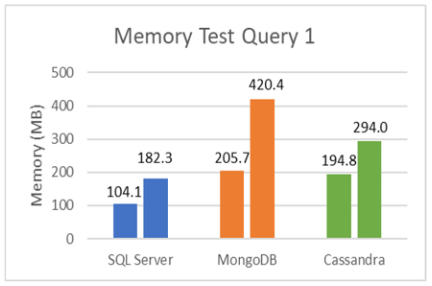
\includegraphics[width=\textwidth]{images/cov19-mem-test-q1.png}
            \caption{Memoria RAM utilizada para la Query 1.}
            \label{cov19-memtest-q1}
        \end{minipage}
        \hfill
        \begin{minipage}[b]{0.48\textwidth}
            \centering
            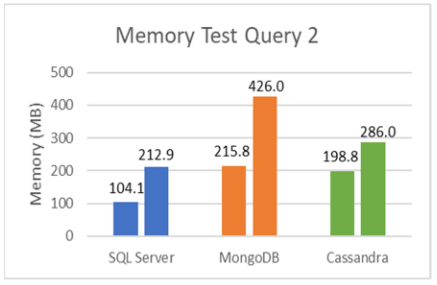
\includegraphics[width=\textwidth]{images/cov19-mem-test-q2.png}
            \caption{Memoria RAM utilizada para la Query 2.}
            \label{cov19-memtest-q2}
        \end{minipage}
    \end{figure}
\end{frame}

\begin{frame}
    \frametitle{Assessment of SQL and NoSQL Systems to Store and Mine COVID-19 Data}

    \begin{figure}[H]
        \centering
        \begin{minipage}[b]{0.48\textwidth}
            \centering
            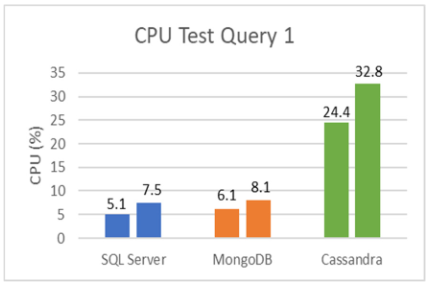
\includegraphics[width=\textwidth]{images/cov19-cpu-test-q1.png}
            \caption{Porcentaje de CPU utilizado para la Query 1.}
            \label{cov19-cputest-q1}
        \end{minipage}
        \hfill
        \begin{minipage}[b]{0.48\textwidth}
            \centering
            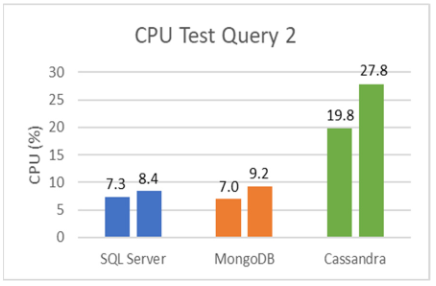
\includegraphics[width=\textwidth]{images/cov19-cpu-test-q2.png}
            \caption{Porcentaje de CPU utilizado para la Query 2.}
            \label{cov19-cputest-q2}
        \end{minipage}
    \end{figure}
\end{frame}

\begin{frame}
    \frametitle{Assessment of SQL and NoSQL Systems to Store and Mine COVID-19 Data}

    \begin{figure}[H]
        \centering
        \begin{minipage}[b]{0.48\textwidth}
            \centering
            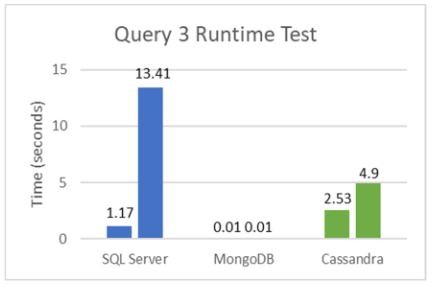
\includegraphics[width=\textwidth]{images/cov19-runt-test-q3.png}
            \caption{Prueba de tiempo de ejecución para la Query 3.}
            \label{cov19-runtest-q3}
        \end{minipage}
        \hfill
        \begin{minipage}[b]{0.48\textwidth}
            \centering
            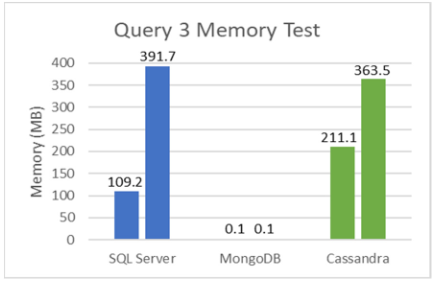
\includegraphics[width=\textwidth]{images/cov19-mem-test-q3.png}
            \caption{Memoria RAM utilizada para la Query 3.}
            \label{cov19-memtest-q3}
        \end{minipage}
    \end{figure}
\end{frame}

\begin{frame}
    \frametitle{Assessment of SQL and NoSQL Systems to Store and Mine COVID-19 Data}

    \begin{figure}[H]
        \centering
        \begin{minipage}[b]{0.48\textwidth}
            \centering
            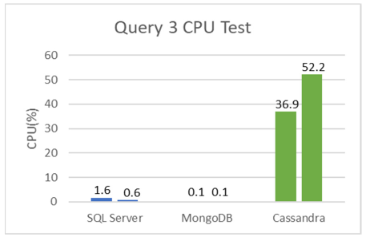
\includegraphics[width=\textwidth]{images/cov19-cpu-test-q3.png}
            \caption{Porcentaje de CPU utilizado para la Query 3.}
            \label{cov19-runtest-q3}
        \end{minipage}
        \hfill
        \begin{minipage}[b]{0.48\textwidth}
            \centering
            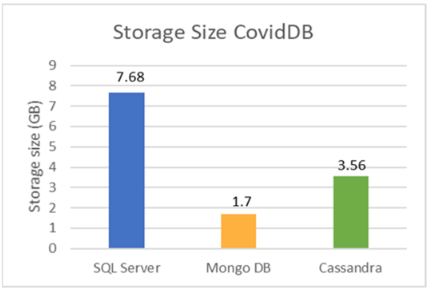
\includegraphics[width=\textwidth]{images/cov19-storage.png}
            \caption{Tamaño de la base de datos de COVID-19.}
            \label{cov19-memtest-q3}
        \end{minipage}
    \end{figure}
\end{frame}

\subsubsection{Conclusiones}

\begin{frame}
    \frametitle{Assessment of SQL and NoSQL Systems to Store and Mine COVID-19 Data - Conclusiones}

    Cabe destacar que los experimentos que no se mostraron, utilizaron consultas con \textit{joins}, y SQL Server tuvo un mejor rendimiento.

     

    \begin{itemize}
        \item SQL Server debería ser la elección si los datos son muy estructurados y necesitan consultas con \textit{joins}.

         
    
        \item Si se utiliza un gran volumen de datos no estructurados y no es necesario realizar demasiadas consultas con \textit{joins}, MongoDB o Cassandra se consideran las soluciones más adecuadas.
    \end{itemize}
\end{frame}